\documentclass[11pt]{article}
\usepackage{../shared/hanzocover}
\usepackage[utf8]{inputenc}
\usepackage[T1]{fontenc}
\usepackage{amsmath,amssymb}
\usepackage{graphicx}
\usepackage{booktabs}
\usepackage{xcolor}
\usepackage{listings}
\input{../shared/lstlang}
\usepackage{tikz}
\usetikzlibrary{shapes,arrows.meta,positioning,fit,backgrounds,calc}
\usepackage[hidelinks]{hyperref}

\definecolor{codegreen}{rgb}{0,0.6,0}
\definecolor{codegray}{rgb}{0.5,0.5,0.5}
\definecolor{codepurple}{rgb}{0.58,0,0.82}
\definecolor{backcolour}{rgb}{0.96,0.96,0.94}
\definecolor{hzblue}{rgb}{0.12,0.30,0.55}
\definecolor{hzslate}{rgb}{0.22,0.25,0.30}
\definecolor{hzgreen}{rgb}{0.10,0.45,0.25}
\definecolor{hzred}{rgb}{0.60,0.16,0.16}

\lstdefinestyle{mystyle}{
    backgroundcolor=\color{backcolour},
    commentstyle=\color{codegreen},
    keywordstyle=\color{codepurple},
    numberstyle=\tiny\color{codegray},
    stringstyle=\color{codegreen},
    basicstyle=\ttfamily\footnotesize,
    breakatwhitespace=false,
    breaklines=true,
    captionpos=b,
    keepspaces=true,
    numbers=none,
    showspaces=false,
    showstringspaces=false,
    showtabs=false,
    tabsize=2,
    frame=single,
    rulecolor=\color{codegray}
}
\lstset{style=mystyle}

\title{Consensus Orders Decisions, Not Bytes: A Plugin-Placement Runtime\\ for a Planet-Scale Multi-Tenant Cloud}
\author{Zach Kelling\thanks{Corresponding author: research@hanzo.ai} \\
    \textit{Hanzo Industries Inc (Techstars '17)} \\
    Los Angeles, California \\
    \texttt{https://hanzo.ai}}
\date{HIP-0116 \quad Revision~1}

\begin{document}

\hanzocoverpage

\twocolumn[
  \begin{@twocolumnfalse}
  \maketitle
  \begin{abstract}
  \noindent
  We describe how the Hanzo unified cloud binary (\texttt{hanzoai/cloud},
  HIP-0106) becomes a \emph{planet-scale, consensus-backed, plugin-placement
  PaaS runtime}: a developer authors a high-performance, ZAP-native plugin in
  minutes---one small interface and one \texttt{cloud.Register} call---and it
  \emph{inherits} placement, per-tenant sharding, streaming replication,
  per-connection pinning, and high availability from the runtime, writing
  none of those mechanisms. The design rests on one decision: \emph{consensus
  orders decisions, not bytes.} A small \emph{post-quantum},
  Byzantine-fault-tolerant replicated state machine (RSM)---the \textbf{Quasar}
  engine (\texttt{luxfi/consensus/protocol/quasar}), strict-PQ from day
  one---over a fixed five-voter quorum orders only tiny
  metadata---membership, a
  placement map $(\textit{plugin},\textit{shard}) \!\to\! \{\textit{writer},
  \textit{followers}\}$, and writer leases carrying fencing epochs---while the
  large byte streams (SQLite WAL, ZapDB deltas) ride the existing,
  \emph{unchanged} asynchronous log-ship data plane (HIP-0107). The two planes
  are decomplected: consensus sits off the request path, so losing the
  control-plane quorum freezes \emph{placement} but not \emph{serving}. This
  is the Chubby / etcd shape---a small strongly-consistent coordination kernel
  steering a large weakly-coupled fleet---applied to a plugin runtime. We give
  the two-plane architecture, the single write-fence seam that couples them,
  a two-fence split-brain-safety argument (a linearizable lease grant
  \emph{and} an object-store epoch compare-and-swap), the five-voter /
  $N$-data-node topology, the plugin-authoring payoff, the
  Deployment$\rightarrow$StatefulSet cutover, and a nine-stage migration in
  which every stage is independently correct, canary-able, and reversible.
  This is a design proposal (HIP-0116, Draft), not a report on a shipped
  system.
  \end{abstract}
  \vspace{1.5em}
  \end{@twocolumnfalse}
]

\section{Introduction}
\label{sec:intro}

The unified cloud binary~\cite{hip0106} collapsed roughly thirty-five
Hanzo Go subsystems into a single statically linked artifact: identity, key
management, an application runtime, a gateway, inference, commerce, storage,
messaging, and observability all mount into one operating-system process, and
inter-subsystem calls are Go function invocations rather than network hops.
That work solved \emph{packaging}---one image, one pipeline, one process to
observe. It did not solve \emph{placement}.

Placement is the question a stateful multi-tenant runtime cannot avoid: for a
given plugin and a given tenant, \emph{which} replica owns the write side of
that state, how is a second replica \emph{prevented} from writing the same
state concurrently, and how does a \emph{new} plugin inherit both without
re-implementing them. Today the Hanzo answer is partial and per-service. Key
management already log-ships an encrypted mirror of its store and fences its
single writer with a Kubernetes Lease object; identity carries an explicit
guard that refuses to run more than one replica; every other stateful
subsystem either reinvents ``who writes'' or runs a single replica and calls
it high availability. A plugin author inherits none of it.

This paper describes the runtime that closes the gap, and the single idea
that makes it small: \textbf{consensus orders decisions, not bytes.} The
observation is that placement is a \emph{tiny, strongly-consistent} decision
problem sitting on top of a \emph{large, already-solved, weakly-consistent}
byte problem. The bytes---write-ahead-log frames and database deltas---are
already handled by one unified replication pipeline~\cite{hip0107}. What is
missing is a single authority that says, linearizably, \emph{who} may push
those bytes for \emph{which} shard at \emph{which} epoch. That authority is a
replicated state machine, and it needs to order only kilobytes of metadata,
never a tenant byte.

We make four claims. First, separating a strongly-consistent
\emph{control plane} from a weakly-consistent \emph{data plane}, and keeping
consensus off the request path, yields a runtime that \emph{degrades in
agility, not availability}, under quorum loss (\S\ref{sec:twoplanes},
\S\ref{sec:failure}). Second, the coupling between the planes is a
\emph{single function}---the write-fence seam---and its safety against
split-brain follows from two independent fences (\S\ref{sec:seam},
\S\ref{sec:failure}). Third, because placement is an inherited property of
plugin registration, a developer gets planet-scale, sharded, replicated, HA
behavior \emph{for free} (\S\ref{sec:dx}). Fourth, the entire change is
migratable in nine stages that are each independently correct, canary-able,
and reversible (\S\ref{sec:migration}). We are explicit throughout about
what we are \emph{not} claiming: this is a design (HIP-0116, Draft), the
consensus engine provides ordering but not the pinned-writer semantics we
build on top, and the compat surface introduced mid-migration is the one
place a bug becomes a cross-tenant breach.

\section{Motivation}
\label{sec:motivation}

\paragraph{Three almost-identical single-writer patterns.}
The status quo is three separate solutions to one problem. Key management
(\texttt{hanzoai/kms}) log-ships its ZapDB store to an age-encrypted
object-store mirror and gates the push loop on a Kubernetes Lease held by
exactly one pod; this works but binds the write path to the Kubernetes API
server, offers one writer for the \emph{whole} service with no per-tenant
sharding, and carries no fencing token beyond the Lease's own renewal.
Identity refuses a second replica outright. The remaining stateful services
run a single replica. Three failure stories, three on-call burdens, and a
hard ceiling of one writer for anything with write state.

\paragraph{Consensus on the data path is the wrong reflex.}
The tempting fix---put every write through a consensus log so all replicas
agree on state---makes consensus a \emph{dependency of serving}. A quorum
loss then stops writes everywhere, and the consensus log must carry the full
byte volume of every tenant's mutations. This is the failure mode we
explicitly reject. A control plane that must be up for the data plane to
serve has simply moved the single point of failure, not removed it.

\paragraph{The Chubby insight.}
Burrows's Chubby lock service~\cite{chubby} and the etcd coordination kernel
that followed~\cite{etcdraft} embody the alternative: a \emph{small}
strongly-consistent service hands out leases and membership, and a
\emph{large} fleet of loosely-coupled workers does the actual work, consulting
the kernel only to learn \emph{who owns what}, not to perform each operation.
The kernel is on the \emph{coordination} path, never the \emph{data} path.
We adopt exactly this shape: the consensus RSM is a lease-and-placement
kernel; the plugins are the loosely-coupled fleet; and a plugin serves every
request against its local state with no consensus round-trip.

\section{Two Planes, Decomplected}
\label{sec:twoplanes}

The load-bearing structural decision is that the control plane and the data
plane never braid. Table~\ref{tab:planes} states the split; consensus orders
the left column and never touches the right.

\begin{table}[h]
\centering
\footnotesize
\caption{The two planes. Consensus orders decisions (left), never bytes (right).}
\label{tab:planes}
\begin{tabular}{@{}p{2.05cm}p{2.55cm}p{2.55cm}@{}}
\toprule
 & \textbf{Control plane} & \textbf{Data plane} \\
\midrule
Orders & placement decisions & durable bytes \\
Substrate & \textbf{Quasar} PQ-BFT RSM (\texttt{luxfi/consensus/protocol/quasar}), 5 voters & \texttt{hanzoai/replicate} over \texttt{vfs}, async log-ship \\
Size & kilobytes (fits in RAM everywhere) & terabytes (per-tenant streams) \\
Consistency & linearizable & eventual to mirror; strong at the writer \\
Request path? & \textbf{no} & \textbf{yes} \\
If it stops & placement frozen, \textbf{serving continues} & shard stalls until a writer is re-placed \\
\bottomrule
\end{tabular}
\end{table}

The consequence is the property that justifies the whole architecture:
because the control plane is \emph{off} the request path, a control-plane
quorum loss is a degradation of \emph{agility}, not \emph{availability}.
Existing writers hold their leases and keep serving reads and writes; only
rebalancing and failover pause until quorum returns. Figure~\ref{fig:topology}
shows the two planes and the one-directional dependence between them: data
nodes \emph{watch} the placement map but never block on the RSM to serve.

\begin{figure*}[t]
\centering
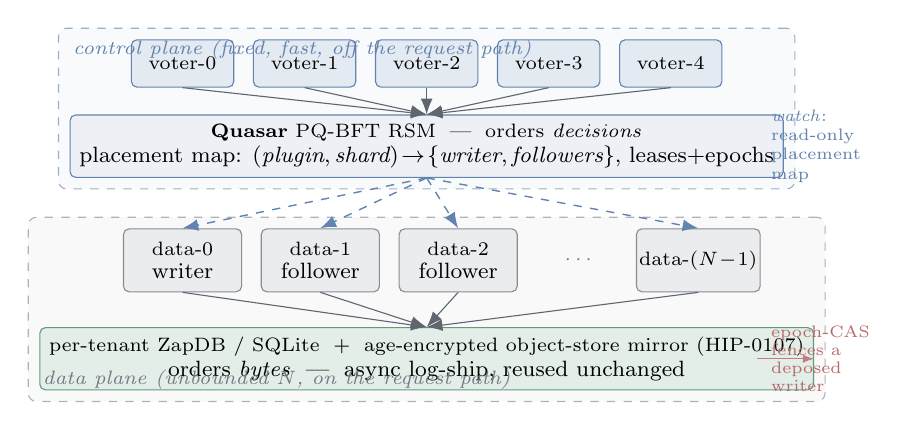
\begin{tikzpicture}[
  font=\scriptsize,
  node distance=5mm,
  voter/.style={draw=hzblue!70, fill=hzblue!12, rounded corners=2pt,
                minimum width=13mm, minimum height=6mm, inner sep=1pt},
  data/.style={draw=hzslate!60, fill=hzslate!10, rounded corners=2pt,
               minimum width=15mm, minimum height=8mm, align=center, inner sep=1pt},
  store/.style={draw=hzgreen!70, fill=hzgreen!12, rounded corners=2pt,
                minimum width=52mm, minimum height=7mm, align=center},
  rsm/.style={draw=hzblue!70, fill=hzblue!8, rounded corners=2pt,
              minimum width=52mm, minimum height=7mm, align=center},
  arr/.style={-{Latex[length=2mm]}, hzslate!80, line width=0.4pt},
  watch/.style={-{Latex[length=2mm]}, hzblue!70, line width=0.5pt, dashed}
]

% --- control plane: five voters + RSM ---
\node[voter] (v0) at (0.0,3.05) {voter-0};
\node[voter] (v1) at (1.55,3.05) {voter-1};
\node[voter] (v2) at (3.10,3.05) {voter-2};
\node[voter] (v3) at (4.65,3.05) {voter-3};
\node[voter] (v4) at (6.20,3.05) {voter-4};

\node[rsm] (rsm) at (3.10,2.0)
  {\textbf{Quasar} PQ-BFT RSM \;---\; orders \emph{decisions}\\[1pt]
   \footnotesize placement map: $(\textit{plugin},\textit{shard})\!\to\!\{\textit{writer},\textit{followers}\}$, leases$+$epochs};

\foreach \v in {v0,v1,v2,v3,v4} { \draw[arr] (\v.south) -- (rsm.north); }

% --- data plane: N data nodes ---
\node[data] (d0) at (0.0,0.55) {data-0\\\footnotesize writer};
\node[data] (d1) at (1.75,0.55) {data-1\\\footnotesize follower};
\node[data] (d2) at (3.50,0.55) {data-2\\\footnotesize follower};
\node[hzslate!70] (ddots) at (5.05,0.55) {$\cdots$};
\node[data] (dn) at (6.55,0.55) {data-$(N\!-\!1)$};

% --- data plane byte sink ---
\node[store] (mirror) at (3.10,-0.7)
  {per-tenant ZapDB / SQLite \;$+$\; age-encrypted object-store mirror (HIP-0107)\\[1pt]
   \footnotesize orders \emph{bytes} \;---\; async log-ship, reused unchanged};

% watch edges (control -> data, read-only)
\foreach \d in {d0,d1,d2,dn} { \draw[watch] (rsm.south) -- (\d.north); }
% data -> sink
\foreach \d in {d0,d1,d2,dn} { \draw[arr] (\d.south) -- (mirror.north); }

% fence annotation on the writer's push
\node[hzred!70, anchor=west, font=\fontsize{5.6}{6.6}\selectfont, align=left]
  at (7.35,-0.7) {epoch-CAS\\fences a\\deposed\\writer};
\draw[-{Latex[length=1.4mm]}, hzred!60] (7.3,-0.7) -- (mirror.east);

\begin{scope}[on background layer]
  \node[draw=hzblue!45, dashed, rounded corners=3pt, fit=(v0)(v4)(rsm),
        inner sep=4pt, fill=hzblue!3] (cp) {};
  \node[draw=hzslate!40, dashed, rounded corners=3pt, fit=(d0)(dn)(mirror),
        inner sep=4pt, fill=hzslate!3] (dp) {};
\end{scope}
\node[hzblue!70, anchor=north west, font=\scriptsize\itshape]
  at ([xshift=2pt,yshift=-1pt]cp.north west) {control plane (fixed, fast, off the request path)};
\node[hzslate!70, anchor=south west, font=\scriptsize\itshape]
  at ([xshift=2pt,yshift=1pt]dp.south west) {data plane (unbounded $N$, on the request path)};

\node[hzblue!70, anchor=west, font=\fontsize{6}{7}\selectfont, align=left]
  at (7.35,2.0) {\emph{watch}:\\read-only\\placement\\map};

\end{tikzpicture}
\caption{The two decomplected planes. A fixed five-voter Quasar post-quantum
BFT replicated state machine orders only \emph{decisions}---membership, the
placement map, and
epoch-fenced writer leases (kilobytes). An unbounded set of data nodes
\emph{watches} a read-only copy of that map and serves the actual
\emph{bytes} through the unchanged asynchronous log-ship pipeline
(HIP-0107). The dependence is one-directional: data nodes read the map but
never block on the control plane to serve, so a control-plane quorum loss
freezes placement while serving continues (\S\ref{sec:twoplanes},
\S\ref{sec:failure}).}
\label{fig:topology}
\end{figure*}


\section{The Control Plane: a Placement RSM}
\label{sec:control}

The control plane is one \textbf{Quasar} replicated state machine---Quasar is
a \emph{post-quantum}, Byzantine-fault-tolerant consensus engine with ordered
finality~\cite{luxconsensus,pulsar}. We choose PQ-BFT finality deliberately:
the decision being ordered is \emph{who is allowed to write}, a wrong or
equivocating answer must be \emph{impossible} rather than merely improbable,
and the lease-granting quorum must itself be quantum-secure on-doctrine. The
RSM drives the engine (\texttt{luxfi/consensus/protocol/quasar}'s
\texttt{NewEngine(cfg)}) through its ordered-finality API---%
\texttt{Submit(block)} appends a placement command,
\texttt{Finalized()} yields the finalized block sequence, and
\texttt{IsFinalized(id)} checks one command---and the placement map is the
state machine built by reducing that finalized sequence. Each finalized block
carries small, idempotent commands---\texttt{Join}, \texttt{Leave},
\texttt{Assign}, \texttt{Revoke}, \texttt{RenewLease},
\texttt{Rebalance}---each naming a plugin, a shard, a node, and a
monotonically increasing fencing epoch. The deterministic reduction of that
sequence is the \emph{placement map}: the current member set and, for every
shard, its writer, its followers, and its epoch.

Two invariants hold by construction. First, \emph{one writer per shard per
epoch}: an \texttt{Assign} for a shard commits only if its epoch strictly
exceeds the shard's current epoch, and because the log is linearizable, two
nodes can never both hold a valid lease for the same shard at the same epoch.
Second, \emph{epochs are monotonic per shard}: a superseded writer's epoch is
permanently in the past and can never be revived. This is the fencing token
the data plane checks.

The RSM log holds \emph{only} this metadata. It never sees a WAL frame, a
secret, or a tenant byte---it is a coordination kernel, not a database. It
\emph{replaces} the interim Kubernetes-Lease fence that key management uses
today: that Lease was always a placeholder for a real distributed lease with
fencing, and the RSM is that lease, carrying an epoch the Kubernetes Lease
never had and depending on no external control plane on the write path.

\paragraph{Post-quantum from day one.}
The engine runs under a strict post-quantum cert profile from the
start---not classical-now / PQ-later. The RSM binds the strict profile via
\texttt{SetProfile(*config.ChainSecurityProfile)}, and the
\texttt{Certifier}'s triple-mode gate (\texttt{demandsTriple}) then requires
the post-quantum certificate before a block finalizes. The threshold signer
is the \emph{Pulsar RoundSigner}
(\texttt{protocol/quasar/pulsar/round\_signer.go}, adapting
\texttt{luxfi/pulsar}~\cite{pulsar}: Pulsar threshold ML-DSA with a Corona
Ring-LWE production threshold), and it fails \emph{closed} to the PQ path
rather than degrading to a classical signature. The quorum that grants a
writer lease is therefore quantum-secure by construction.

\paragraph{Full Byzantine agreement across $N$ voters.}
The quorum shape is decided: the control plane runs true $N$-node Byzantine
agreement, not crash-fault replication. Each finalized block is certified by a
threshold signature whose shares are split across the voter pods and
aggregated through the Pulsar RoundSigner's
\texttt{Round1}\,/\,\texttt{Round2}\,/\,\texttt{Finalize} protocol carried over
ZAP~\cite{hip0114}; every voter then independently verifies the aggregated
post-quantum certificate before applying the finalized block to its
placement-map state machine. A block lacking a valid triple-mode certificate
never finalizes, so a Byzantine minority of voters can neither forge a
placement decision nor equivocate a lease grant. Byzantine tolerance and the
strict post-quantum certificate are orthogonal and both on from day one: the
first is \emph{how many} faulty voters are survived, the second is \emph{what}
signs the result.

\paragraph{What Quasar provides, and what it does not.}
Quasar supplies native membership (a validator-set manager per network
identifier); a totally ordered, finalized command stream through
\texttt{NewEngine}\,/\,\texttt{Submit}\,/\,\texttt{Finalized}\,/\,\texttt{IsFinalized};
post-quantum BFT finality gated by the \texttt{ChainSecurityProfile} and
certified by the Pulsar RoundSigner; and a pure-Go embed that links into the
same static binary with \texttt{CGO\_ENABLED=0}. It does \emph{not} provide a
pinned-writer primitive: Quasar is
leaderless by design~\cite{avalanche}, with no built-in notion of ``this node
leads this key.'' \textbf{The host builds writer-pinning on top, as RSM
leases}---and that construction, the placement map and its epoch-fenced
assignments, is precisely the contribution of this work. Quasar gives
ordered, post-quantum agreement; the \emph{meaning} of the ordered commands
is ours.

\paragraph{An honest dependency prerequisite.}
The strict-PQ path does not build from published module tags today, and we do
not present it as if it does. The threshold-signature primitive the adapter
consumes is published (\texttt{luxfi/pulsar}, the \texttt{ref/go/pkg/pulsar}
RoundSigner, at v1.1.5), and the base \texttt{protocol/quasar} engine is
published; the gap is a single consensus-side release. The cert-profile
sub-package \texttt{protocol/quasar/pulsar}---the \texttt{PulsarRoundSigner}
adapter---is unpublished, present in none of the \texttt{luxfi/consensus}
release tags and carried only on a development branch behind a \texttt{replace}
directive that Go ignores for downstream consumers. The prerequisite is thus
one \texttt{luxfi/consensus} release tag that includes
\texttt{protocol/quasar/pulsar}, requires the published \texttt{luxfi/pulsar}
v1.1.5, and drops the development \texttt{replace}---a forward-port in
progress. Until it lands, the control plane compiles the strict-PQ path only
against local checkouts. We state this because a proposal that hid a real,
unmet build prerequisite would be dishonest about its own readiness.

\section{The Data Plane, and the One Seam}
\label{sec:seam}

The data plane is the existing unified replication pipeline~\cite{hip0107},
reused \emph{verbatim}: a source adapter pumps frames, an age
layer~\cite{age} encrypts them at the boundary, and a virtual-file-system
backend writes them to an encrypted object-store mirror. Nothing about the
byte path changes---same frames, same encryption, same bucket layout, same
recovery objectives. Key management already runs exactly this loop against
ZapDB.

The entire coupling between the two planes is a \emph{single function}. Today
the primary's push gate asks whether it holds the Kubernetes Lease. Under
this design it asks whether the control plane grants \emph{this shard's} lease
at the current epoch, and every push additionally performs a compare-and-swap
on the mirror's recorded fencing epoch:

\begin{lstlisting}[language=Go]
// today (interim): hold the K8s Lease?
func canPush(h *atomic.Bool, f *writerLease) bool {
    return h.Load() && f.Held()
}

// proposed: does the RSM grant THIS shard at
// epoch E?  ... and the mirror CAS must accept E.
func canPush(h *atomic.Bool, g LeaseGrant) bool {
    return h.Load() && g.Valid()
}
// each push: succeed iff mirrorEpoch <= g.Epoch,
// then advance mirrorEpoch := g.Epoch
\end{lstlisting}

This gives two independent fences, defense in depth. The \emph{RSM grant} is
a linearizable, in-memory check: a node pushes only for shards the placement
map says it writes, at the current epoch. The \emph{object-store epoch-CAS}
is a durable check at the sink: even a partitioned node that still
\emph{believes} it holds the lease loses the compare-and-swap against a
\texttt{latest} pointer already advanced by its successor. A deposed writer
\emph{physically cannot} append to the shared log. We make the safety
consequence precise in \S\ref{sec:failure}.

\section{Topology}
\label{sec:topology}

The fleet is five voter nodes and $N$ non-voting data nodes. Five is the
smallest quorum with Byzantine finality tolerating two simultaneous failures;
the count is \emph{fixed} so agreement stays fast---consensus runs among five,
not among the whole fleet. Each data node watches a read-only replica of the
placement map (the RSM streams committed updates to it), hosts the shards the
map assigns, runs the unchanged replication loop, and serves or proxies
requests. Data nodes carry no consensus weight, so $N$ scales \emph{unbounded}
without slowing agreement. In small deployments a node may be both voter and
data node; at scale they separate so control-plane latency is independent of
data-plane fan-out. The defaults are five voters and three data replicas---one
writer plus two warm standbys, tolerating one node loss with a ready
successor.

\section{Placement Unit and Sharding}
\label{sec:shard}

The unit of placement is the \emph{plugin}---exactly the
$(\textit{name},\textit{order},\textit{fn})$ triple registered through
\texttt{cloud.Register}---crossed with a \emph{shard}. Version one ships
\emph{coarse}: the shard is the whole plugin, one global writer per plugin
behind which every tenant's data lives. This is \emph{zero storage change}---the
plugin's existing single data directory \emph{is} the single shard, and it is
the key-management shape today generalized to every plugin. A later, opt-in
refinement makes the shard $(\textit{plugin},\textit{org})$, giving per-tenant
writers over the per-organization file layout~\cite{hip0302} that already
exists, so a hot tenant earns its own writer while a cold tenant costs
nothing until touched.

Node \emph{specialization} is expressed two ways, both orthogonal to code.
\emph{Which shards live where} is the placement map---dynamic, moved by the
RSM at runtime; this is failover and rebalancing. \emph{Which plugins a
node-pool may run at all} is the static per-pool enabled-subsystem
set~\cite{hip0106}, for resource isolation. Specialization is \emph{never} a
runtime mount or unmount of plugin code: every binary contains every compiled
plugin, and placement decides which \emph{shards} are \emph{active} where, not
which \emph{code} is \emph{present}. One artifact, many roles, by data rather
than by rebuild.

\section{Per-Connection Pinning}
\label{sec:pinning}

Routing a connection to the byte-owner is one middleware, mounted immediately
after the identity middleware so it runs with a validated organization already
in context. It computes the shard from the plugin and the organization, looks
up the owner in the watched, in-memory placement map with no RPC, and then:
serves locally if this node is the writer; reverse-proxies to the writer for a
write or a read-your-writes read; and serves from a local follower, or proxies
to any follower, for an explicitly stale-tolerant read.
Figure~\ref{fig:pinning} shows the path. Proxying is pod-to-pod over the
StatefulSet headless service---a node dials its peer directly by stable DNS
name, with no load balancer in the middle and no extra ingress hop. The client
sees one endpoint; the fleet routes the connection to the byte-owner
underneath.

\begin{figure}[t]
\centering
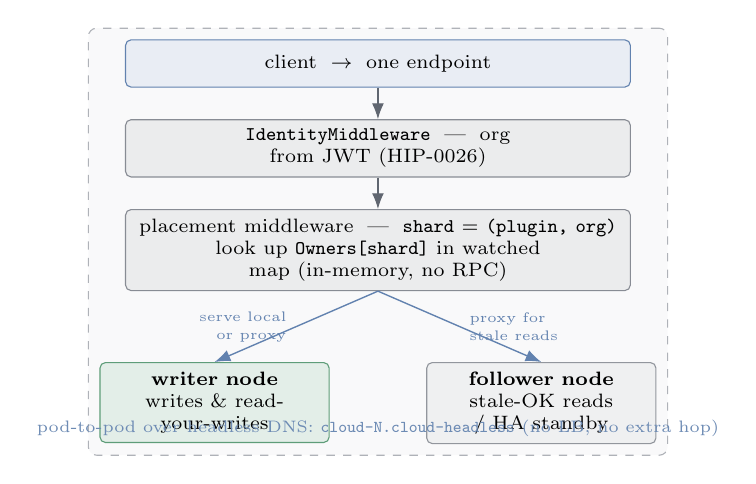
\begin{tikzpicture}[
  font=\scriptsize,
  node distance=4mm,
  box/.style={draw, rounded corners=2pt, align=center, minimum height=6mm,
              inner xsep=3pt, text width=62mm},
  edge/.style={box, fill=hzblue!10, draw=hzblue!70},
  mid/.style={box, fill=hzslate!10, draw=hzslate!60},
  writer/.style={box, fill=hzgreen!12, draw=hzgreen!70, text width=27mm},
  follow/.style={box, fill=hzslate!8, draw=hzslate!55, text width=27mm},
  arr/.style={-{Latex[length=2mm]}, hzslate!80, line width=0.4pt},
  proxy/.style={-{Latex[length=2mm]}, hzblue!70, line width=0.5pt}
]

\node[edge] (client) {client \;$\rightarrow$\; one endpoint};
\node[mid, below=of client] (ident) {\texttt{IdentityMiddleware} \;---\; org from JWT (HIP-0026)};
\node[mid, below=of ident] (pin)
  {placement middleware \;---\; \texttt{shard $=$ (plugin, org)}\\
   look up \texttt{Owners[shard]} in watched map (in-memory, no RPC)};

\node[writer, below left=9mm and -26mm of pin] (w)
  {\textbf{writer node}\\ writes \& read-your-writes};
\node[follow, below right=9mm and -26mm of pin] (f)
  {\textbf{follower node}\\ stale-OK reads / HA standby};

\draw[arr] (client) -- (ident);
\draw[arr] (ident) -- (pin);
\draw[proxy] (pin.south) -- node[left, font=\fontsize{5.5}{6.5}\selectfont, hzblue!70,align=right]
  {serve local\\ or proxy} (w.north);
\draw[proxy] (pin.south) -- node[right, font=\fontsize{5.5}{6.5}\selectfont, hzblue!70,align=left]
  {proxy for\\ stale reads} (f.north);

\node[hzblue!65, anchor=north, font=\fontsize{5.6}{6.6}\selectfont]
  at ([yshift=-1mm]$(w)!0.5!(f)$)
  {pod-to-pod over headless DNS: \texttt{cloud-N.cloud-headless} (no LB, no extra hop)};

\begin{scope}[on background layer]
  \node[draw=hzslate!40, dashed, rounded corners=3pt, fit=(client)(ident)(pin)(w)(f),
        inner sep=4pt, fill=hzslate!3] (b) {};
\end{scope}

\end{tikzpicture}
\caption{Per-connection pinning. The placement middleware mounts immediately
after identity resolution, computes the shard from plugin and organization,
resolves the owner from the watched placement map with no round-trip, and
either serves locally or reverse-proxies pod-to-pod over the StatefulSet
headless service to the shard's writer (writes, read-your-writes) or a
follower (stale-tolerant reads). The client sees one endpoint
(\S\ref{sec:pinning}).}
\label{fig:pinning}
\end{figure}


\section{The Payoff: Authoring a Plugin}
\label{sec:dx}

The purpose of the runtime is what a developer does \emph{not} have to write.
A plugin author implements one small interface and one \texttt{cloud.Register}
call and \emph{inherits} consensus placement, per-tenant sharding, shared
replication, per-connection pinning, and high availability. The default wire
is ZAP-native~\cite{hip0114}, high-performance by construction---the
object-storage subsystem is already ZAP-native with a gRPC call count of
zero, and key management runs a ZAP server today---so a new plugin gets that
transport with no extra work. A complete ``hello, sharded, replicated,
highly-available plugin'' is about twenty lines:

\begin{lstlisting}[language=Go]
package hello

import (
    "github.com/hanzoai/cloud"
    "github.com/hanzoai/zip"
)

type Store struct{ db cloud.ShardDB }

func mount(app *zip.App, deps cloud.Deps) error {
    s := &Store{db: deps.OpenShard("hello")}
    app.Get("/v1/hello/:key", func(c zip.Ctx) error {
        return c.JSON(s.db.Get(c.Param("key")))
    })
    app.Put("/v1/hello/:key", func(c zip.Ctx) error {
        return s.db.Put(c.Param("key"), c.Body())
    })
    return nil
}

func init() { cloud.Register("hello", 500, mount) }
\end{lstlisting}

Everything the author did not write, but got: the RSM chose which node writes
\texttt{hello}; the pinning middleware routed each connection to it; the
replication loop mirrored the store to encrypted object storage; a follower
stands ready for promotion on writer loss; and the epoch fence guarantees no
split-brain write. The plugin is planet-scale and highly available because it
was \emph{registered}, not because it was \emph{engineered} to be. This is the
same economy the unified binary~\cite{hip0106} gave inter-subsystem calls and
the extension runtime~\cite{hip0105} gave user code, extended to stateful
placement.

\section{Deployment: Deployment $\rightarrow$ StatefulSet}
\label{sec:deploy}

The runtime needs stable identity---a node's identifier must survive a restart
so RSM membership and the placement map stay valid---and stable storage---a
node must reopen the same shard files. That is a StatefulSet, not a
Deployment. The workload moves from a single-replica Deployment with the
Recreate strategy to an $N$-replica StatefulSet with stable ordinal
identifiers, a headless service for pod-to-pod dialing, per-pod persistent
volume claims via volume-claim templates, and a rolling update with at most
one pod unavailable in ordered-ready mode.

The decisive property is that stable identifiers make a rolling image upgrade
\emph{not} a membership change: the RSM sees the same five voters and the same
data-node identities before and after, so no epoch reconfiguration and no
placement churn occur on a deploy, and at-most-one-unavailable keeps the
four-of-five voter quorum live throughout. The existing service aliases keep
resolving because the StatefulSet pods still carry the selector label the
aliases match. The operator's service custom resource~\cite{hip0112} gains a
StatefulSet-emitting mode---one boolean that switches the render path from a
Deployment to a StatefulSet with a headless service and volume-claim
templates---leaving the resource contract otherwise unchanged.

\section{Migration}
\label{sec:migration}

The change reaches production in nine stages. Every stage is independently
correct, can be canaried, and is reversible; none requires a flag day.

\begin{enumerate}\itemsep2pt
\item \textbf{Dependencies and inert config.} Vendor the pure-Go consensus
engine and add the placement types and knobs \emph{compiled in but inert}.
Nothing behaves differently.
\item \textbf{RSM in shadow.} Mount the placement RSM as its own subsystem
running in shadow: the voters agree a placement map and data nodes watch it,
but nothing consults it yet---verify in production that the shadow map matches
the live Lease holder before trusting it.
\item \textbf{Flip the fence seam.} Point the push gate at the RSM grant and
add the object-store epoch-CAS, keeping the Kubernetes-Lease path behind a
flag for one release so the cutover is a reversible toggle. This is the single
highest-value edit.
\item \textbf{Operator emits StatefulSet.} Teach the service custom resource
the StatefulSet mode and migrate key management's workload to it, still at one
replica---this stage changes only the \emph{kind}.
\item \textbf{Key management beyond one replica, coarse.} Raise to multiple
replicas with the whole service as one coarse shard: one elected writer, the
rest followers, pinning live. Prove failover by killing the writer and
watching a follower take the next epoch while the object-store CAS fences the
old one.
\item \textbf{Retire the external secret store.} Import and verify every
secret by count and checksum; stand up a compatibility shim for legacy
clients---\emph{this shim is the cross-tenant-leak surface and the primary
adversarial-review target of the entire migration}---verify the deprecation
gates and machine identities, then decommission the old store.
\item \textbf{Roll coarse writers to the remaining stateful services.} Bring
tasks, publish-subscribe, and the SQLite-backed services under coarse
placement. The audit service specifically must move its in-memory sequence
counter to the replicated store \emph{before} it can have a second replica,
lest two writers mint colliding sequence numbers.
\item \textbf{Identity beyond one replica.} Last, because it is the highest
blast radius: move sessions to a replicated shard, hold a single signing key
set in key management, and lift the one-replica guard identity carries today.
\item \textbf{Fine per-tenant sharding.} Split coarse plugin-shards into
per-tenant shards on the per-organization layout, opt-in per plugin. This is a
placement-map refinement---a finer shard key, no new mechanism---and is
explicitly future work.
\end{enumerate}

\section{Safety and Failure Modes}
\label{sec:failure}

\paragraph{No two writers (split-brain safety).}
For any shard and any wall-clock instant, at most one node holds a valid lease
grant. The argument has two independent fences. The RSM commits an assignment
for a shard only with an epoch strictly greater than the shard's current
epoch, and its log is linearizable, so no two valid grants share a shard and
epoch. Independently, a push to the mirror succeeds only if its epoch is at
least the mirror's recorded epoch, which each successful writer advances
monotonically; a partitioned ex-writer carrying a stale epoch $e' < e$ is
rejected at the compare-and-swap even if it never learned it was deposed.
Either fence alone prevents corruption of the shared log; together they are
defense in depth.

\paragraph{Control-plane quorum loss.}
With three or more voters down, placement is frozen: no new failovers, no
rebalancing. Serving continues, because consensus is off the data path and
every data node already caches the last-known-good placement map. Agility
degrades; availability does not.

\paragraph{Writer node loss.}
The RSM assigns the shard to a follower at the next epoch; the follower, which
has been replicating the shard, is promoted by a placement-map update rather
than a data copy, and pinning re-routes new connections to it.

\paragraph{Rolling upgrade and migration correctness.}
Stable identifiers make an image roll invisible to the RSM---no epoch
reconfiguration, no churn---while at-most-one-unavailable preserves quorum.
Every data migration, whether the coarse-to-fine split or the external-store
import, is verified by count and checksum before the old source is retired; no
cutover trusts the copy. The one genuinely dangerous surface is the
compatibility shim of stage six: it translates legacy paths into
organization-scoped lookups, and a scoping bug there leaks another tenant's
secret. It is called out as the primary adversarial-review target precisely
because it is the one place a bug becomes a breach rather than an outage.

\section{Decided Forks}
\label{sec:forks}

We record the choices and their rationale. Quasar PQ-BFT for the control
plane---\emph{full $N$-node Byzantine agreement} (decided, not crash-fault):
threshold shares split across voter pods, aggregated via the Pulsar RoundSigner
\texttt{Round1}/\texttt{Round2}/\texttt{Finalize} over ZAP, each voter
verifying the aggregated certificate before applying a finalized block---because
a lease grant must be impossible to forge or equivocate, not merely unlikely.
\emph{Strict post-quantum from day one} (the Pulsar RoundSigner under a strict
\texttt{ChainSecurityProfile}), orthogonal to and simultaneous with the
Byzantine guarantee, never classical-now / PQ-later, so the lease-granting
quorum is quantum-secure on-doctrine from the start. Five
voters plus $N$ data nodes, the smallest
Byzantine quorum tolerating two failures, with unbounded data-node fan-out.
Coarse per-plugin sharding first, because one writer per plugin is
\emph{zero} storage change; fine per-tenant sharding is a later opt-in. The
writer serves reads and followers are HA standbys, the simplest correct
default, with follower-served stale reads available per connection for
read-heavy plugins. Asynchronous log-ship as the default replication mode,
reusing the existing pipeline unchanged, with synchronous zero-RPO
replication a \emph{per-shard} opt-in rather than a fleet-wide tax. Defaults
of five voters and three data replicas.

\section{What We Do Not Claim}
\label{sec:notclaim}

This is a design proposal, not a report on a deployed system; the nine stages
are the plan by which it would ship. The consensus engine provides ordering
and membership, not the pinned-writer semantics---those are built on top, and
their correctness is ours to defend, not the engine's. The runtime does not
put consensus on the request path and therefore does not give
consensus-consistency to \emph{reads}: a stale-tolerant read from a follower
is exactly that. It is not a general scheduler---coarse placement of plugins
onto pools remains the operator's job. And it does not fold the payment-card
systems, which stay their own deployments under the solo-vault
rule~\cite{hip0106}. The saving is not that consensus made everything
consistent; it is that consensus was confined to the one small thing that
needed it, and kept away from the large thing that did not.

\section{Related Work}
\label{sec:related}

The architecture is the Chubby lock service~\cite{chubby} and the etcd
coordination kernel~\cite{etcdraft} in shape: a small strongly-consistent
service for leases and membership, consulted for \emph{who owns what} and
never on the data path. Our leases carry fencing tokens in the sense
Kleppmann describes for correct distributed locking~\cite{fencing}---the epoch
is the token, and the object-store compare-and-swap is the resource-side check
that makes the token effective against a delayed writer. The ordering
substrate is a \emph{post-quantum} Byzantine-fault-tolerant replicated
state machine in the lineage of Practical BFT~\cite{pbft}, realized as the
leaderless Quasar engine~\cite{avalanche,luxconsensus} with a Pulsar
threshold-signature cert profile~\cite{pulsar} that makes the lease-granting
quorum quantum-secure; the state-machine-replication framing is the classical
one~\cite{smr}. The byte
plane is log-shipping in the Litestream lineage~\cite{litestream} unified
under one pipeline~\cite{hip0107}. Where we differ from a database that puts
every write through consensus (in the Raft~\cite{raft} or Paxos~\cite{paxos}
tradition) is precisely the decomplection: we order the placement decision,
not the mutation, so the byte volume never touches the consensus log and
serving never blocks on quorum.

\section{Conclusion}
\label{sec:conclusion}

A stateful multi-tenant runtime has to answer who writes what, prevent two
writers from racing, and let a new plugin inherit both. The naive answer puts
every write through consensus and makes the coordinator a new single point of
failure. The answer here is to notice that placement is a tiny,
strongly-consistent decision on top of a large, already-solved,
weakly-consistent byte stream, and to order only the decision. A five-voter
BFT replicated state machine holds membership, a placement map, and
epoch-fenced writer leases; the existing asynchronous log-ship carries the
bytes unchanged; and a single write-fence seam, guarded by a linearizable
grant and an object-store epoch compare-and-swap, couples them safely. The
control plane sits off the request path, so quorum loss costs agility, not
availability. The payoff is that a developer authoring a ZAP-native plugin in
minutes inherits placement, sharding, replication, pinning, and high
availability by registering it. Consensus earns its keep by doing one small
thing well and staying out of everything else.

{\small
\bibliographystyle{plain}
\bibliography{references}
}

\end{document}
